\documentclass[11pt]{article}

% Change "review" to "final" to generate the final (sometimes called camera-ready) version.
% Change to "preprint" to generate a non-anonymous version with page numbers.
\usepackage{acl}

% Standard package includes
\usepackage{times}
\usepackage{latexsym}

% For proper rendering and hyphenation of words containing Latin characters (including in bib files)
\usepackage[T1]{fontenc}
% For Vietnamese characters
% \usepackage[T5]{fontenc}
% See https://www.latex-project.org/help/documentation/encguide.pdf for other character sets

% This assumes your files are encoded as UTF8
\usepackage[utf8]{inputenc}

% This is not strictly necessary, and may be commented out,
% but it will improve the layout of the manuscript,
% and will typically save some space.
\usepackage{microtype}

% This is also not strictly necessary, and may be commented out.
% However, it will improve the aesthetics of text in
% the typewriter font.
\usepackage{inconsolata}

%Including images in your LaTeX document requires adding
%additional package(s)
\usepackage{graphicx}

\title{Project 1}

\author{Jesus Soto Gonzalez \\
  \texttt{jhsoto@iastate.edu}}

\begin{document}

\maketitle

\begin{abstract}
This first project for COM S 5790, Natural Language Processing applies basic NLP and word embedding methods 
to a given dataset. We preprocessed the text by tokenizing it, removing stopwords, and using phrase mining. 
From this, we created frequency- and TF--IDF-based word clouds to highlight key terms. 
For semantic analysis, we trained Word2Vec models on both words and phrases to find the nearest neighbors 
of top TF--IDF terms. Phrase mining with \texttt{gensim}'s bigram and trigram models helped capture multiword 
expressions and produced clearer, more meaningful embeddings.
\end{abstract}

\section{Methods}

\subsection{Preprocessing}
The dataset was first filtered to only include abstracts with Category = 1. 
Each abstract was sentence-split, tokenized, lowercased, and cleaned by removing stopwords and non-alphabetic 
tokens using NLTK. The result was saved both as plain text for word clouds and as token lists in JSON for 
Word2Vec tasks respectively.

\subsection{Phrase Mining}
To capture multiword terms, I used the \texttt{gensim} library for phrase mining. 
I first trained a bigram model on the tokenized corpus with a minimum count of 8 and a threshold of 8.0. 
This combined pairs of words that often appeared together. 
Then, I trained a trigram model on top of the bigrams to join longer expressions. 
In both cases, phrases were written with underscores, such as \textit{carcass\_composition}, 
\textit{average\_daily\_gain}, and \textit{backfat\_thickness}.  

I also tested different parameter values. 
Stricter settings 10, 10.0 created fewer but very strong phrases, while looser ones 5, 5.0 or 3, 3.0 
created more phrases but added noise. The balanced setting 8, 8.0 worked best, since it kept important 
domain phrases like \textit{quantitative\_trait\_locus} and \textit{meat\_quality} without introducing too 
many random ones. This choice was important because phrase quality directly influenced the TF--IDF terms 
and the results from Word2Vec.

\subsection{TF--IDF and Word Clouds}
From both the unigram and phrased corpus I computed frequency counts and TF--IDF scores. 
The top-ranked terms were visualized as word clouds, which made it easy to compare terms that 
are simply common versus those that are more distinctive.

\subsection{Word2Vec}
I trained Word2Vec models on both the words and phrased corpus using CBOW with a vector size of 100, a window of 5,
and a minimum count of 10 as required. Then, to evaluate the models, I looked at the nearest neighbors of the 
top TF--IDF terms and compared how the results changed when using phrases instead of single words.

\section{Main Results}

\subsection{Word Clouds -- Task 1}
The frequency-based word cloud was dominated by very common research terms such as \textit{qtl}, 
\textit{traits}, \textit{study}, and \textit{genes}. These words appear often across many abstracts but do not 
point to specific findings. In contrast, the TF--IDF word cloud highlighted more distinctive domain terms, 
including \textit{ascites}, \textit{earlobe}, \textit{pleurisy}, and \textit{ketosis}. This shows how TF--IDF can 
surface technical vocabulary that is less frequent overall but more informative for understanding the dataset. 

\begin{figure}[h]
  \centering
  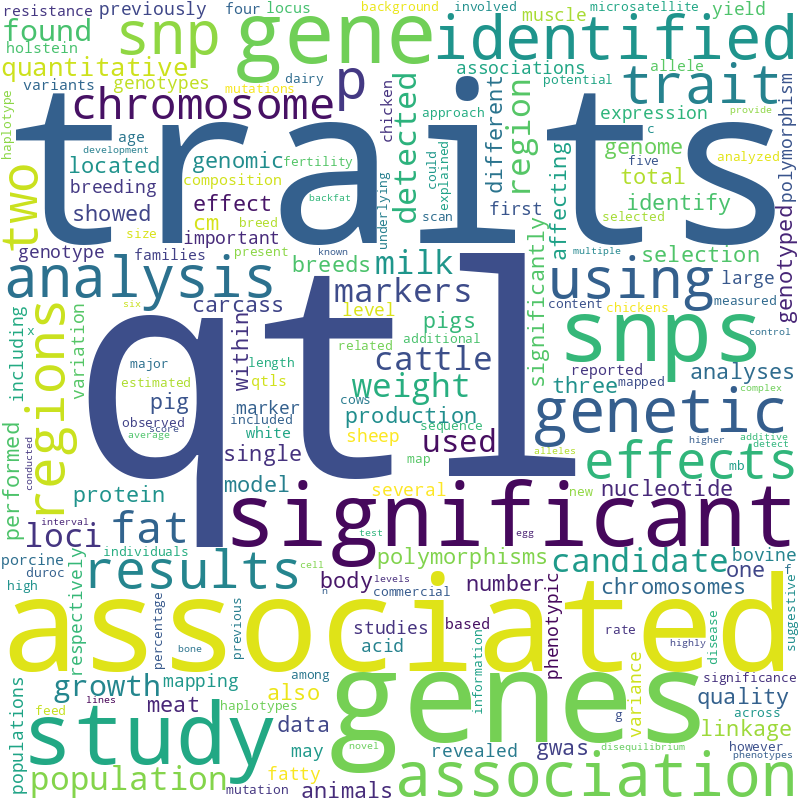
\includegraphics[width=0.8\linewidth]{../outputs/freq_wordcloud_task1.png}
  \caption{Task 1 frequency-based word cloud. Common words such as \textit{qtl} and \textit{traits} dominate.}
  \label{fig:freq_wc_task1}
\end{figure}

\begin{figure}[h]
  \centering
  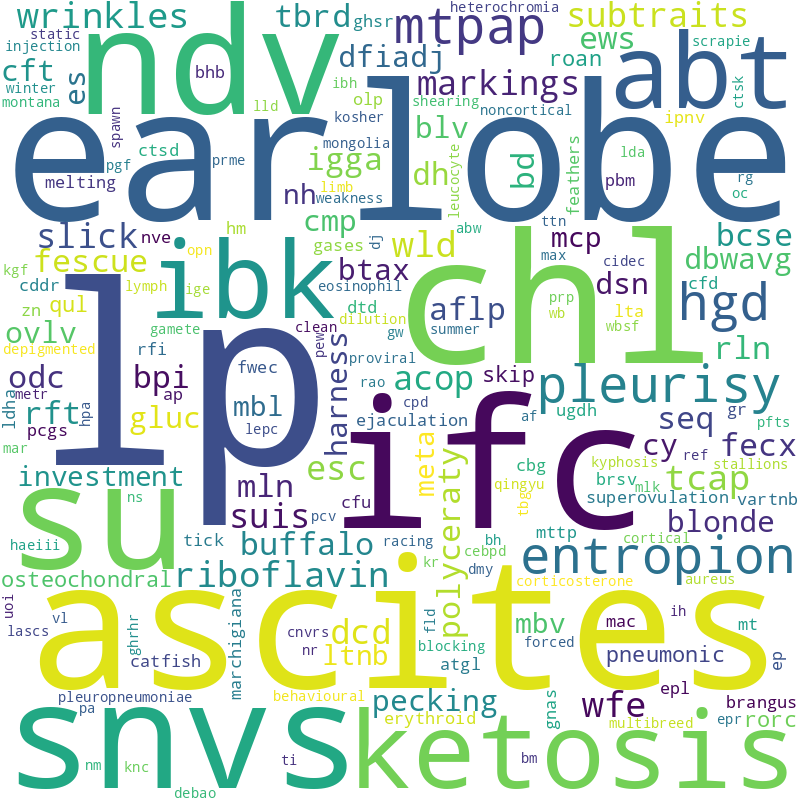
\includegraphics[width=0.8\linewidth]{../outputs/tfidf_wordcloud_task1.png}
  \caption{Task 1 TF--IDF-based word cloud. Distinctive domain terms like \textit{ascites} and \textit{earlobe} stand out.}
  \label{fig:tfidf_wc_task1}
\end{figure}


\section{Preamble}

The first line of the file must be
\begin{quote}
\begin{verbatim}
\documentclass[11pt]{article}
\end{verbatim}
\end{quote}

To load the style file in the review version:
\begin{quote}
\begin{verbatim}
\usepackage[review]{acl}
\end{verbatim}
\end{quote}
For the final version, omit the \verb|review| option:
\begin{quote}
\begin{verbatim}
\usepackage{acl}
\end{verbatim}
\end{quote}

To use Times Roman, put the following in the preamble:
\begin{quote}
\begin{verbatim}
\usepackage{times}
\end{verbatim}
\end{quote}
(Alternatives like txfonts or newtx are also acceptable.)

Please see the \LaTeX{} source of this document for comments on other packages that may be useful.

Set the title and author using \verb|\title| and \verb|\author|. Within the author list, format multiple authors using \verb|\and| and \verb|\And| and \verb|\AND|; please see the \LaTeX{} source for examples.

By default, the box containing the title and author names is set to the minimum of 5 cm. If you need more space, include the following in the preamble:
\begin{quote}
\begin{verbatim}
\setlength\titlebox{<dim>}
\end{verbatim}
\end{quote}
where \verb|<dim>| is replaced with a length. Do not set this length smaller than 5 cm.

\section{Document Body}

\subsection{Footnotes}

Footnotes are inserted with the \verb|\footnote| command.\footnote{This is a footnote.}

\subsection{Tables and figures}

See Table~\ref{tab:accents} for an example of a table and its caption.
\textbf{Do not override the default caption sizes.}

\begin{table}
  \centering
  \begin{tabular}{lc}
    \hline
    \textbf{Command} & \textbf{Output} \\
    \hline
    \verb|{\"a}|     & {\"a}           \\
    \verb|{\^e}|     & {\^e}           \\
    \verb|{\`i}|     & {\`i}           \\
    \verb|{\.I}|     & {\.I}           \\
    \verb|{\o}|      & {\o}            \\
    \verb|{\'u}|     & {\'u}           \\
    \verb|{\aa}|     & {\aa}           \\\hline
  \end{tabular}
  \begin{tabular}{lc}
    \hline
    \textbf{Command} & \textbf{Output} \\
    \hline
    \verb|{\c c}|    & {\c c}          \\
    \verb|{\u g}|    & {\u g}          \\
    \verb|{\l}|      & {\l}            \\
    \verb|{\~n}|     & {\~n}           \\
    \verb|{\H o}|    & {\H o}          \\
    \verb|{\v r}|    & {\v r}          \\
    \verb|{\ss}|     & {\ss}           \\
    \hline
  \end{tabular}
  \caption{Example commands for accented characters, to be used in, \emph{e.g.}, Bib\TeX{} entries.}
  \label{tab:accents}
\end{table}

As much as possible, fonts in figures should conform
to the document fonts. See Figure~\ref{fig:experiments} for an example of a figure and its caption.

Using the \verb|graphicx| package graphics files can be included within figure
environment at an appropriate point within the text.
The \verb|graphicx| package supports various optional arguments to control the
appearance of the figure.
You must include it explicitly in the \LaTeX{} preamble (after the
\verb|\documentclass| declaration and before \verb|\begin{document}|) using
\verb|\usepackage{graphicx}|.

\begin{figure}[t]
  \includegraphics[width=\columnwidth]{example-image-golden}
  \caption{A figure with a caption that runs for more than one line.
    Example image is usually available through the \texttt{mwe} package
    without even mentioning it in the preamble.}
  \label{fig:experiments}
\end{figure}

\begin{figure*}[t]
  \includegraphics[width=0.48\linewidth]{example-image-a} \hfill
  \includegraphics[width=0.48\linewidth]{example-image-b}
  \caption {A minimal working example to demonstrate how to place
    two images side-by-side.}
\end{figure*}

\subsection{Hyperlinks}

Users of older versions of \LaTeX{} may encounter the following error during compilation:
\begin{quote}
\verb|\pdfendlink| ended up in different nesting level than \verb|\pdfstartlink|.
\end{quote}
This happens when pdf\LaTeX{} is used and a citation splits across a page boundary. The best way to fix this is to upgrade \LaTeX{} to 2018-12-01 or later.

\subsection{Citations}

\begin{table*}
  \centering
  \begin{tabular}{lll}
    \hline
    \textbf{Output}           & \textbf{natbib command} & \textbf{ACL only command} \\
    \hline
    \citep{Gusfield:97}       & \verb|\citep|           &                           \\
    \citealp{Gusfield:97}     & \verb|\citealp|         &                           \\
    \citet{Gusfield:97}       & \verb|\citet|           &                           \\
    \citeyearpar{Gusfield:97} & \verb|\citeyearpar|     &                           \\
    \citeposs{Gusfield:97}    &                         & \verb|\citeposs|          \\
    \hline
  \end{tabular}
  \caption{\label{citation-guide}
    Citation commands supported by the style file.
    The style is based on the natbib package and supports all natbib citation commands.
    It also supports commands defined in previous ACL style files for compatibility.
  }
\end{table*}

Table~\ref{citation-guide} shows the syntax supported by the style files.
We encourage you to use the natbib styles.
You can use the command \verb|\citet| (cite in text) to get ``author (year)'' citations, like this citation to a paper by \citet{Gusfield:97}.
You can use the command \verb|\citep| (cite in parentheses) to get ``(author, year)'' citations \citep{Gusfield:97}.
You can use the command \verb|\citealp| (alternative cite without parentheses) to get ``author, year'' citations, which is useful for using citations within parentheses (e.g. \citealp{Gusfield:97}).

A possessive citation can be made with the command \verb|\citeposs|.
This is not a standard natbib command, so it is generally not compatible
with other style files.

\subsection{References}

\nocite{Ando2005,andrew2007scalable,rasooli-tetrault-2015}

The \LaTeX{} and Bib\TeX{} style files provided roughly follow the American Psychological Association format.
If your own bib file is named \texttt{custom.bib}, then placing the following before any appendices in your \LaTeX{} file will generate the references section for you:
\begin{quote}
\begin{verbatim}
\bibliography{custom}
\end{verbatim}
\end{quote}

You can obtain the complete ACL Anthology as a Bib\TeX{} file from \url{https://aclweb.org/anthology/anthology.bib.gz}.
To include both the Anthology and your own .bib file, use the following instead of the above.
\begin{quote}
\begin{verbatim}
\bibliography{anthology,custom}
\end{verbatim}
\end{quote}

Please see Section~\ref{sec:bibtex} for information on preparing Bib\TeX{} files.

\subsection{Equations}

An example equation is shown below:
\begin{equation}
  \label{eq:example}
  A = \pi r^2
\end{equation}

Labels for equation numbers, sections, subsections, figures and tables
are all defined with the \verb|\label{label}| command and cross references
to them are made with the \verb|\ref{label}| command.

This an example cross-reference to Equation~\ref{eq:example}.

\subsection{Appendices}

Use \verb|\appendix| before any appendix section to switch the section numbering over to letters. See Appendix~\ref{sec:appendix} for an example.

\section{Bib\TeX{} Files}
\label{sec:bibtex}

Unicode cannot be used in Bib\TeX{} entries, and some ways of typing special characters can disrupt Bib\TeX's alphabetization. The recommended way of typing special characters is shown in Table~\ref{tab:accents}.

Please ensure that Bib\TeX{} records contain DOIs or URLs when possible, and for all the ACL materials that you reference.
Use the \verb|doi| field for DOIs and the \verb|url| field for URLs.
If a Bib\TeX{} entry has a URL or DOI field, the paper title in the references section will appear as a hyperlink to the paper, using the hyperref \LaTeX{} package.

\section*{Limitations}

This document does not cover the content requirements for ACL or any
other specific venue.  Check the author instructions for
information on
maximum page lengths, the required ``Limitations'' section,
and so on.

\section*{Acknowledgments}

This document has been adapted
by Steven Bethard, Ryan Cotterell and Rui Yan
from the instructions for earlier ACL and NAACL proceedings, including those for
ACL 2019 by Douwe Kiela and Ivan Vuli\'{c},
NAACL 2019 by Stephanie Lukin and Alla Roskovskaya,
ACL 2018 by Shay Cohen, Kevin Gimpel, and Wei Lu,
NAACL 2018 by Margaret Mitchell and Stephanie Lukin,
Bib\TeX{} suggestions for (NA)ACL 2017/2018 from Jason Eisner,
ACL 2017 by Dan Gildea and Min-Yen Kan,
NAACL 2017 by Margaret Mitchell,
ACL 2012 by Maggie Li and Michael White,
ACL 2010 by Jing-Shin Chang and Philipp Koehn,
ACL 2008 by Johanna D. Moore, Simone Teufel, James Allan, and Sadaoki Furui,
ACL 2005 by Hwee Tou Ng and Kemal Oflazer,
ACL 2002 by Eugene Charniak and Dekang Lin,
and earlier ACL and EACL formats written by several people, including
John Chen, Henry S. Thompson and Donald Walker.
Additional elements were taken from the formatting instructions of the \emph{International Joint Conference on Artificial Intelligence} and the \emph{Conference on Computer Vision and Pattern Recognition}.

% Bibliography entries for the entire Anthology, followed by custom entries
%\bibliography{anthology,custom}
% Custom bibliography entries only
\bibliography{custom}

\appendix

\section{Example Appendix}
\label{sec:appendix}

This is an appendix.

\end{document}